% Evaluation Agreement Patterns
% Use with: % Evaluation Agreement Patterns
% Use with: % Evaluation Agreement Patterns
% Use with: % Evaluation Agreement Patterns
% Use with: \input{figures/agreement.tex}

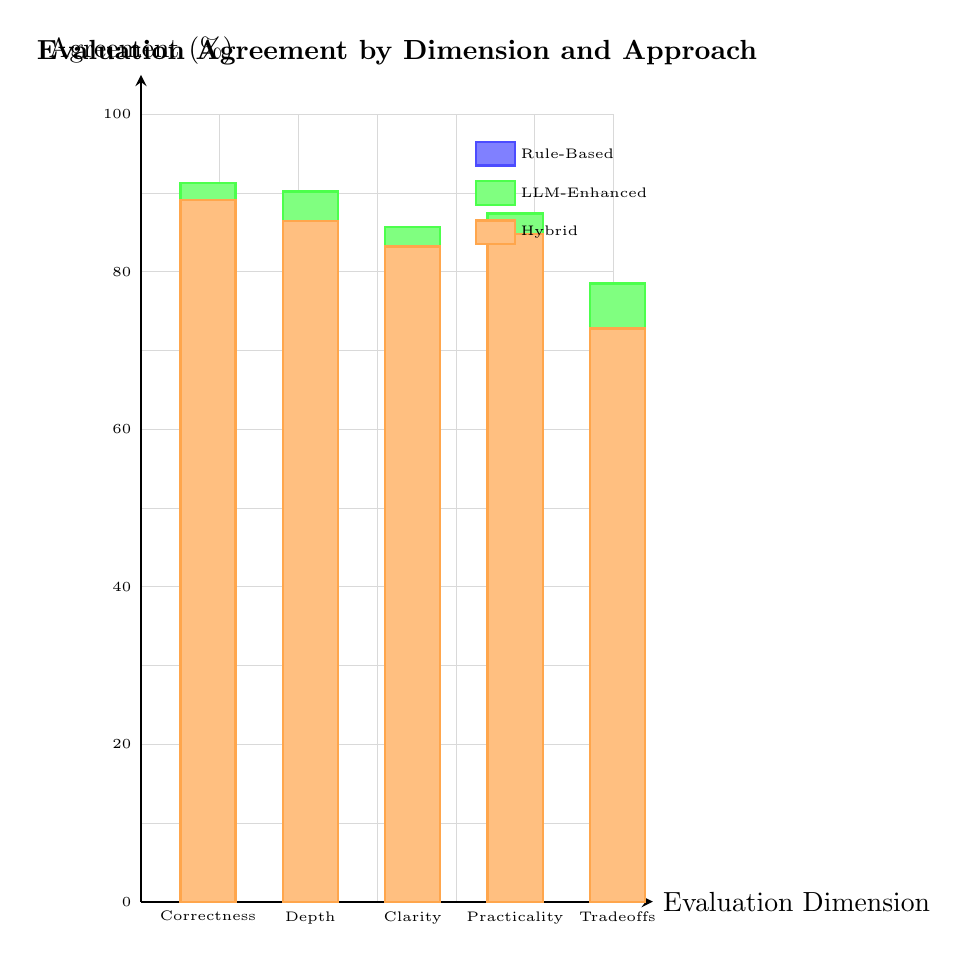
\begin{tikzpicture}[
    axis/.style={->, >=stealth, thick},
    grid/.style={gray!30, very thin},
    bar1/.style={fill=blue!50, draw=blue!70, thick},
    bar2/.style={fill=green!50, draw=green!70, thick},
    bar3/.style={fill=orange!50, draw=orange!70, thick}
]

% Draw grid
\draw[grid] (0,0) grid (6,10);

% Axes
\draw[axis] (0,0) -- (6.5,0) node[right] {Evaluation Dimension};
\draw[axis] (0,0) -- (0,10.5) node[above] {Agreement (\%)};

% Y-axis labels
\foreach \y in {0,20,40,60,80,100}
    \draw (0,\y/10) node[left] {\tiny \y};

% Bars for Rule-Based
\draw[bar1] (0.5,0) rectangle (1.2,7.63);
\draw[bar1] (1.8,0) rectangle (2.5,7.41);
\draw[bar1] (3.1,0) rectangle (3.8,7.89);
\draw[bar1] (4.4,0) rectangle (5.1,7.56);
\draw[bar1] (5.7,0) rectangle (6.4,5.71);

% Bars for LLM-Enhanced
\draw[bar2] (0.5,0) rectangle (1.2,9.13);
\draw[bar2] (1.8,0) rectangle (2.5,9.02);
\draw[bar2] (3.1,0) rectangle (3.8,8.57);
\draw[bar2] (4.4,0) rectangle (5.1,8.74);
\draw[bar2] (5.7,0) rectangle (6.4,7.85);

% Bars for Hybrid
\draw[bar3] (0.5,0) rectangle (1.2,8.91);
\draw[bar3] (1.8,0) rectangle (2.5,8.64);
\draw[bar3] (3.1,0) rectangle (3.8,8.32);
\draw[bar3] (4.4,0) rectangle (5.1,8.48);
\draw[bar3] (5.7,0) rectangle (6.4,7.28);

% X-axis labels
\node[below] at (0.85,0) {\tiny Correctness};
\node[below] at (2.15,0) {\tiny Depth};
\node[below] at (3.45,0) {\tiny Clarity};
\node[below] at (4.75,0) {\tiny Practicality};
\node[below] at (6.05,0) {\tiny Tradeoffs};

% Legend
\node[bar1, minimum width=0.5cm, minimum height=0.3cm] at (4.5,9.5) {};
\node[right] at (4.7,9.5) {\tiny Rule-Based};
\node[bar2, minimum width=0.5cm, minimum height=0.3cm] at (4.5,9) {};
\node[right] at (4.7,9) {\tiny LLM-Enhanced};
\node[bar3, minimum width=0.5cm, minimum height=0.3cm] at (4.5,8.5) {};
\node[right] at (4.7,8.5) {\tiny Hybrid};

% Title
\node[above] at (3.25,10.5) {\textbf{Evaluation Agreement by Dimension and Approach}};

\end{tikzpicture}



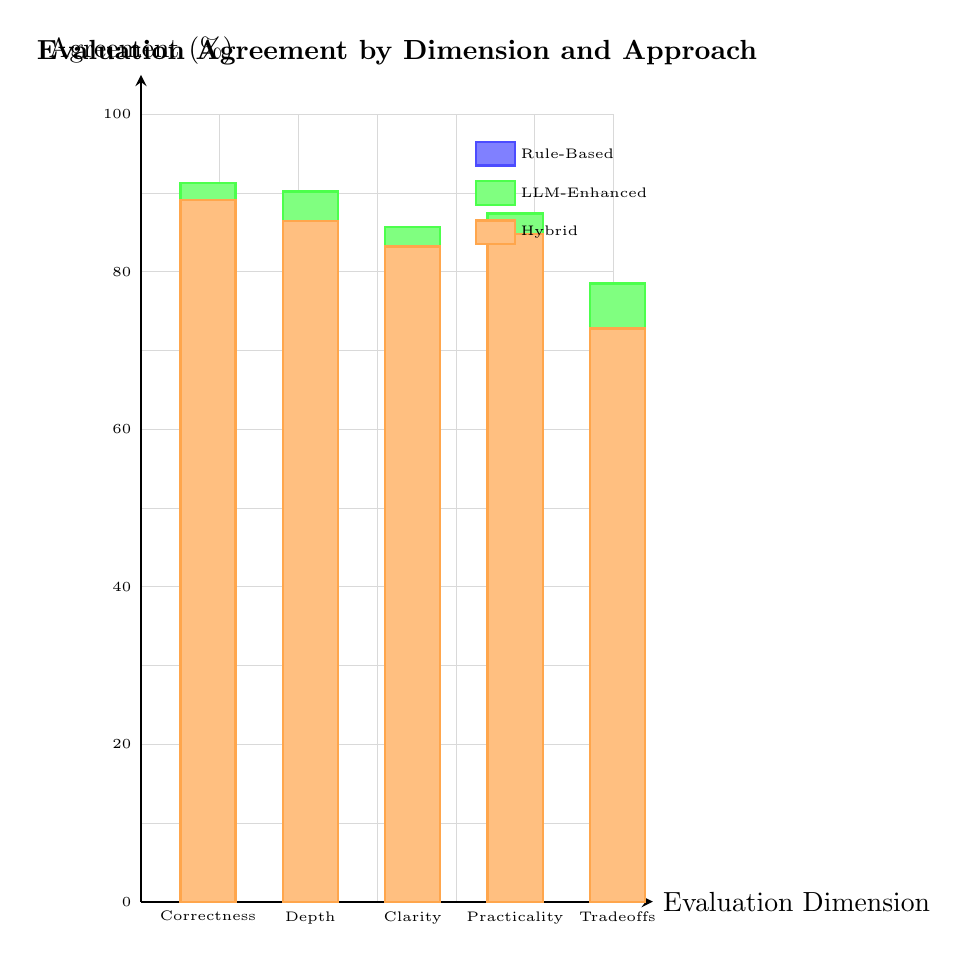
\begin{tikzpicture}[
    axis/.style={->, >=stealth, thick},
    grid/.style={gray!30, very thin},
    bar1/.style={fill=blue!50, draw=blue!70, thick},
    bar2/.style={fill=green!50, draw=green!70, thick},
    bar3/.style={fill=orange!50, draw=orange!70, thick}
]

% Draw grid
\draw[grid] (0,0) grid (6,10);

% Axes
\draw[axis] (0,0) -- (6.5,0) node[right] {Evaluation Dimension};
\draw[axis] (0,0) -- (0,10.5) node[above] {Agreement (\%)};

% Y-axis labels
\foreach \y in {0,20,40,60,80,100}
    \draw (0,\y/10) node[left] {\tiny \y};

% Bars for Rule-Based
\draw[bar1] (0.5,0) rectangle (1.2,7.63);
\draw[bar1] (1.8,0) rectangle (2.5,7.41);
\draw[bar1] (3.1,0) rectangle (3.8,7.89);
\draw[bar1] (4.4,0) rectangle (5.1,7.56);
\draw[bar1] (5.7,0) rectangle (6.4,5.71);

% Bars for LLM-Enhanced
\draw[bar2] (0.5,0) rectangle (1.2,9.13);
\draw[bar2] (1.8,0) rectangle (2.5,9.02);
\draw[bar2] (3.1,0) rectangle (3.8,8.57);
\draw[bar2] (4.4,0) rectangle (5.1,8.74);
\draw[bar2] (5.7,0) rectangle (6.4,7.85);

% Bars for Hybrid
\draw[bar3] (0.5,0) rectangle (1.2,8.91);
\draw[bar3] (1.8,0) rectangle (2.5,8.64);
\draw[bar3] (3.1,0) rectangle (3.8,8.32);
\draw[bar3] (4.4,0) rectangle (5.1,8.48);
\draw[bar3] (5.7,0) rectangle (6.4,7.28);

% X-axis labels
\node[below] at (0.85,0) {\tiny Correctness};
\node[below] at (2.15,0) {\tiny Depth};
\node[below] at (3.45,0) {\tiny Clarity};
\node[below] at (4.75,0) {\tiny Practicality};
\node[below] at (6.05,0) {\tiny Tradeoffs};

% Legend
\node[bar1, minimum width=0.5cm, minimum height=0.3cm] at (4.5,9.5) {};
\node[right] at (4.7,9.5) {\tiny Rule-Based};
\node[bar2, minimum width=0.5cm, minimum height=0.3cm] at (4.5,9) {};
\node[right] at (4.7,9) {\tiny LLM-Enhanced};
\node[bar3, minimum width=0.5cm, minimum height=0.3cm] at (4.5,8.5) {};
\node[right] at (4.7,8.5) {\tiny Hybrid};

% Title
\node[above] at (3.25,10.5) {\textbf{Evaluation Agreement by Dimension and Approach}};

\end{tikzpicture}



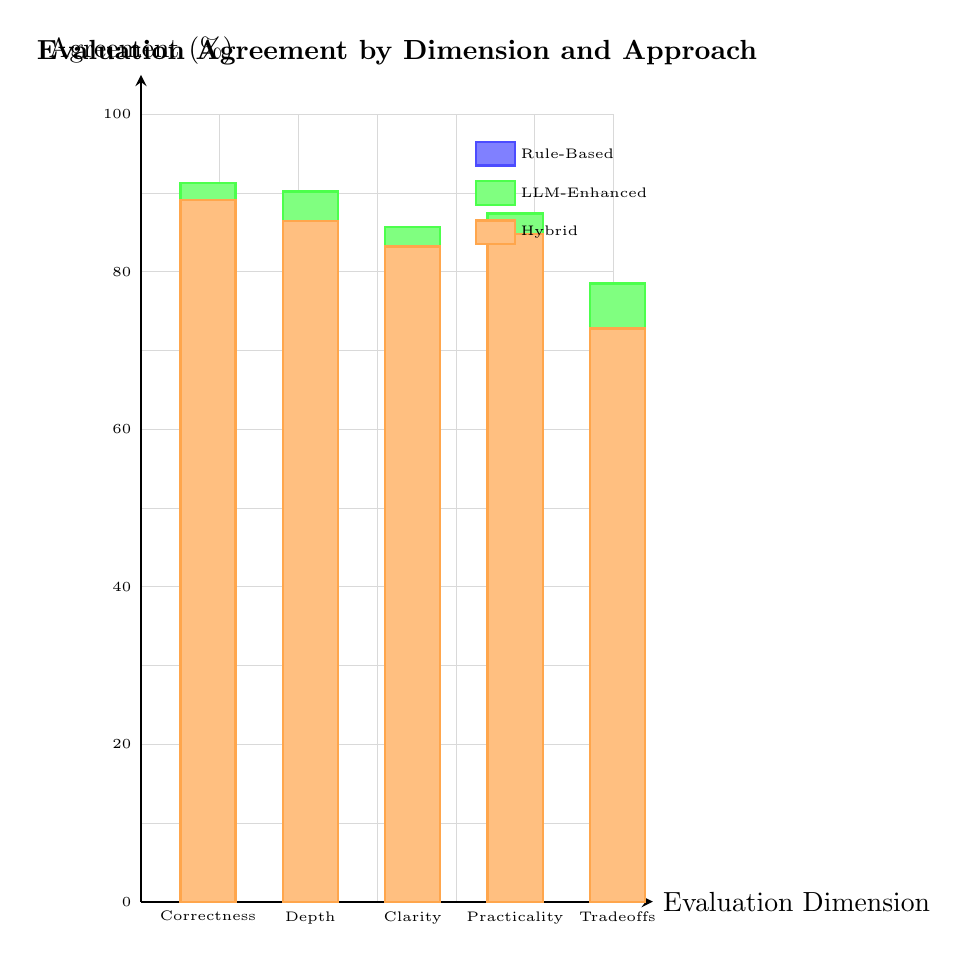
\begin{tikzpicture}[
    axis/.style={->, >=stealth, thick},
    grid/.style={gray!30, very thin},
    bar1/.style={fill=blue!50, draw=blue!70, thick},
    bar2/.style={fill=green!50, draw=green!70, thick},
    bar3/.style={fill=orange!50, draw=orange!70, thick}
]

% Draw grid
\draw[grid] (0,0) grid (6,10);

% Axes
\draw[axis] (0,0) -- (6.5,0) node[right] {Evaluation Dimension};
\draw[axis] (0,0) -- (0,10.5) node[above] {Agreement (\%)};

% Y-axis labels
\foreach \y in {0,20,40,60,80,100}
    \draw (0,\y/10) node[left] {\tiny \y};

% Bars for Rule-Based
\draw[bar1] (0.5,0) rectangle (1.2,7.63);
\draw[bar1] (1.8,0) rectangle (2.5,7.41);
\draw[bar1] (3.1,0) rectangle (3.8,7.89);
\draw[bar1] (4.4,0) rectangle (5.1,7.56);
\draw[bar1] (5.7,0) rectangle (6.4,5.71);

% Bars for LLM-Enhanced
\draw[bar2] (0.5,0) rectangle (1.2,9.13);
\draw[bar2] (1.8,0) rectangle (2.5,9.02);
\draw[bar2] (3.1,0) rectangle (3.8,8.57);
\draw[bar2] (4.4,0) rectangle (5.1,8.74);
\draw[bar2] (5.7,0) rectangle (6.4,7.85);

% Bars for Hybrid
\draw[bar3] (0.5,0) rectangle (1.2,8.91);
\draw[bar3] (1.8,0) rectangle (2.5,8.64);
\draw[bar3] (3.1,0) rectangle (3.8,8.32);
\draw[bar3] (4.4,0) rectangle (5.1,8.48);
\draw[bar3] (5.7,0) rectangle (6.4,7.28);

% X-axis labels
\node[below] at (0.85,0) {\tiny Correctness};
\node[below] at (2.15,0) {\tiny Depth};
\node[below] at (3.45,0) {\tiny Clarity};
\node[below] at (4.75,0) {\tiny Practicality};
\node[below] at (6.05,0) {\tiny Tradeoffs};

% Legend
\node[bar1, minimum width=0.5cm, minimum height=0.3cm] at (4.5,9.5) {};
\node[right] at (4.7,9.5) {\tiny Rule-Based};
\node[bar2, minimum width=0.5cm, minimum height=0.3cm] at (4.5,9) {};
\node[right] at (4.7,9) {\tiny LLM-Enhanced};
\node[bar3, minimum width=0.5cm, minimum height=0.3cm] at (4.5,8.5) {};
\node[right] at (4.7,8.5) {\tiny Hybrid};

% Title
\node[above] at (3.25,10.5) {\textbf{Evaluation Agreement by Dimension and Approach}};

\end{tikzpicture}



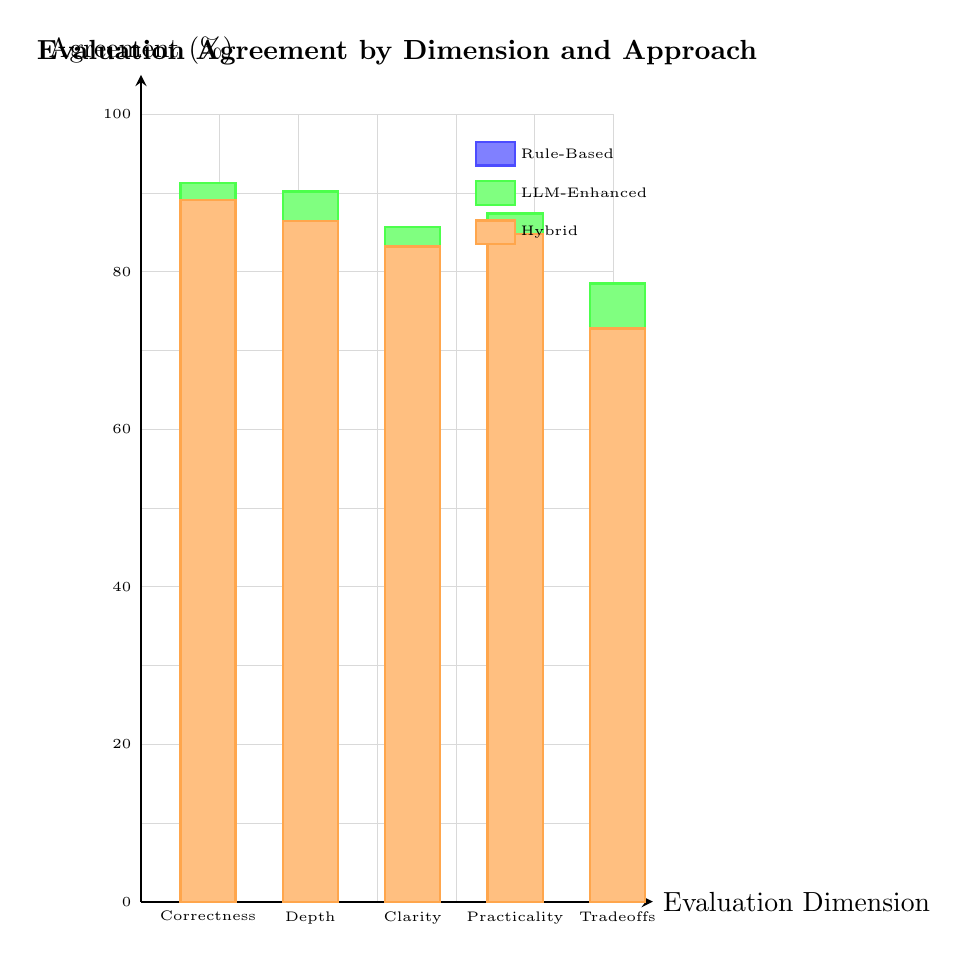
\begin{tikzpicture}[
    axis/.style={->, >=stealth, thick},
    grid/.style={gray!30, very thin},
    bar1/.style={fill=blue!50, draw=blue!70, thick},
    bar2/.style={fill=green!50, draw=green!70, thick},
    bar3/.style={fill=orange!50, draw=orange!70, thick}
]

% Draw grid
\draw[grid] (0,0) grid (6,10);

% Axes
\draw[axis] (0,0) -- (6.5,0) node[right] {Evaluation Dimension};
\draw[axis] (0,0) -- (0,10.5) node[above] {Agreement (\%)};

% Y-axis labels
\foreach \y in {0,20,40,60,80,100}
    \draw (0,\y/10) node[left] {\tiny \y};

% Bars for Rule-Based
\draw[bar1] (0.5,0) rectangle (1.2,7.63);
\draw[bar1] (1.8,0) rectangle (2.5,7.41);
\draw[bar1] (3.1,0) rectangle (3.8,7.89);
\draw[bar1] (4.4,0) rectangle (5.1,7.56);
\draw[bar1] (5.7,0) rectangle (6.4,5.71);

% Bars for LLM-Enhanced
\draw[bar2] (0.5,0) rectangle (1.2,9.13);
\draw[bar2] (1.8,0) rectangle (2.5,9.02);
\draw[bar2] (3.1,0) rectangle (3.8,8.57);
\draw[bar2] (4.4,0) rectangle (5.1,8.74);
\draw[bar2] (5.7,0) rectangle (6.4,7.85);

% Bars for Hybrid
\draw[bar3] (0.5,0) rectangle (1.2,8.91);
\draw[bar3] (1.8,0) rectangle (2.5,8.64);
\draw[bar3] (3.1,0) rectangle (3.8,8.32);
\draw[bar3] (4.4,0) rectangle (5.1,8.48);
\draw[bar3] (5.7,0) rectangle (6.4,7.28);

% X-axis labels
\node[below] at (0.85,0) {\tiny Correctness};
\node[below] at (2.15,0) {\tiny Depth};
\node[below] at (3.45,0) {\tiny Clarity};
\node[below] at (4.75,0) {\tiny Practicality};
\node[below] at (6.05,0) {\tiny Tradeoffs};

% Legend
\node[bar1, minimum width=0.5cm, minimum height=0.3cm] at (4.5,9.5) {};
\node[right] at (4.7,9.5) {\tiny Rule-Based};
\node[bar2, minimum width=0.5cm, minimum height=0.3cm] at (4.5,9) {};
\node[right] at (4.7,9) {\tiny LLM-Enhanced};
\node[bar3, minimum width=0.5cm, minimum height=0.3cm] at (4.5,8.5) {};
\node[right] at (4.7,8.5) {\tiny Hybrid};

% Title
\node[above] at (3.25,10.5) {\textbf{Evaluation Agreement by Dimension and Approach}};

\end{tikzpicture}

